% Diseño digital. Introducción, explicación del protocolo (ya está en la 
% intro), arquitectura del chip, microarquitectura de cada bloque, 
% simulación, biblioteca estándar utilizada, síntesis y place and route. 
% Funciones desarrolladas para simular el diseño.
\chapter{Diseño digital}

El chip cuenta con un bloque digital que realiza un procesamiento 
mínimo de los datos recibidos para presentarlos en forma cruda 
---decodificados y desencapsulados--- en la interfaz digital de 
salida, donde serán utilizados por otros sistemas. Por otro lado 
también realiza el encapsulamiento y codificación de los datos a enviar 
a través del canal de RF,  generando para ello la señal de mando del 
bloque <<Modulador>>. Todo el procesamiento, desde las entradas 
hasta las salidas del bloque digital, se realiza utilizando lógica 
CMOS estática y es sincrónico con la señal portadora de 
\SI{13.56}{\mega\hertz} recibida en la antena. Sin embargo, dado 
que existen pausas en la portadora, el bloque digital también cuenta 
con un pequeño módulo asincrónico que ayuda a decodificar los datos 
recibidos.

El sistema digital fue diseñado utilizando el lenguaje descriptor de 
hardware \emph{Verilog} \cite{Verilog}, con el que se escribieron y 
probaron cada uno de los bloques por separado y luego todos en 
conjunto. La simulación del funcionamiento se realizó utilizando el 
software compilador/sintetizador \emph{Icarus Verilog} \cite{IVerilog} 
junto con \emph{GTKwave} \cite{GTKWave} para visualizar 
los resultados. La implementación del sistema digital fue realizada 
utilizando las herramientas de \emph{Synopsys Inc.} para síntesis (
\emph{Desing Compiler} \cite{SynopsysDC}) y place\&route (\emph{IC 
compiler} \cite{SynopsysICCompiler}), junto con la biblioteca de 
compuertas digitales de la Oklahoma State University (OSU) 
\cite{OSUstandardCells}. 

Para la verificación del funcionamiento a nivel lógico de cada uno 
de los bloques se desarrolló una estructura de pruebas que permitió enviar todas las combinaciones posibles de 
un byte de datos y comprobar su correcta recepción y transmisión. La 
estructura de pruebas consistió en varios \emph{tasks} de Verilog 
parametrizados de forma tal de poder indicar los datos a enviar.

En este capítulo se describirá la arquitectura del sistema digital y su 
funcionamiento. Se analizarán los módulos que conforman el bloque 
digital, su interconexión y se detallará el funcionamiento de cada uno 
de los ellos junto con las simulaciones realizadas. Por último se 
darán detalles acerca de la implementación con las herramientas de 
\emph{Synopsys}.


\section{Arquitectura}

\begin{figure}
	\centering
	\includegraphics[width=\textwidth]{DigitalBlockDiagram}
	\caption{Diagrama en bloques del sistema digital.}
	\label{fig:DigitalBlockDiagram}
\end{figure}

En la figura \ref{fig:DigitalBlockDiagram} se muestra un diagrama en 
bloques del sistema digital. El mismo puede dividirse en dos grandes 
partes que funcionan de forma independiente. Por un lado se 
tienen los módulos que conforman el bloque receptor de datos, 
compuesto por \lstinline{Bit Decoder} y \lstinline{Frame Receiver}, 
donde el primero identifica el comienzo de una trama y decodifica 
los bits recibidos, mientras que el segundo toma los bits 
decodificados y realiza la comprobación de las tramas, esto es, 
comprueba los bits de <<Inicio>>, <<Fin>> y <<Paridad>>. La carga 
útil dentro del frame es transmitida en serie a través de la salida 
\lstinline{rx_bit}, con \lstinline{rx_new_bit} señalizando el 
momento en que el dato es válido.

La recepción de datos se realiza a través de la entrada 
\lstinline{pause}, que es la señal de salida del detector de envolvente
y que se muestrea a una velocidad adecuada como para identificar cada 
bit. 

Por otro lado se tiene el bloque transmisor de datos, formado por 
\lstinline{Tx Buffer}, \lstinline{Frame Sender},
\lstinline{Frame Delay Counter} y \lstinline{Bit Encoder}. Los datos a 
transmitir a través de la interfaz de RF se ingresan en serie al 
buffer \lstinline{Tx Buffer} utilizando las entradas \lstinline{tx_bit}
y \lstinline{tx_new_bit}. El bloque transmisor permite ingresar de uno a 
ocho bits, que serán transmitidos encapsulados en una trama estándar 
luego de cumplido el tiempo de demora FDT. El módulo 
\lstinline{Frame Sender} es el encargado de agregar los bits de 
<<Inicio>>, <<Paridad>> y <<Fin>> correspondientes a la trama e 
iniciar la transmisión cuando recibe la señal del módulo 
\lstinline{Frame Delay Counter}. Los bits a transmitir son codificados 
en formato \emph{Manchester} por el módulo \lstinline{Bit Encoder} 
cuya función es también realizar la modulación OOK (ASK 100\%) con la 
señal sub-portadora de frecuencia \(\sfrac{f_{c}}{16}\). La salida 
\lstinline{coded_out} es la señal codificada y modulada que se conecta 
directamente al circuito modulador de carga.

La transmisión a través de la interfaz de RF debe comenzar luego de
transcurrida una cantidad exacta de ciclos de la señal portadora, 
comenzando a contar a partir de la recepción del símbolo de <<Fin>> 
de trama, según fue definido por el estándar y se vio en la figura 
\ref{fig:EsquemaFDT_PCD_PICC}. El módulo \lstinline{Frame Delay Counter}
se encarga de contar la cantidad de ciclos transcurridos a partir de que
se activa la señal \lstinline{rx_eof}, la cual señaliza el fin de trama 
(\emph{end of frame}), y al cumplirse el tiempo FDT activa la señal 
\lstinline{fdt} que habilita al bloque \lstinline{Frame Sender} a 
iniciar la transmisión. 
	
La señal portadora fue utilizada como reloj para el sistema digital, 
lo que tiene la ventaja de evitar el uso de un generador de reloj 
interno a la vez que sincroniza el transponder con el lector. Sin 
embargo, también tiene la desventaja de que la señal se interrumpe 
debido al esquema de codificación y modulación definido por el 
estándar (sección \ref{sec:ISO14443_2}). Entonces surge el 
inconveniente de que la señal \lstinline{pause} debe ser muestreada 
para decodificar los bits justo en el instante en que no hay reloj. 
Para superar este inconveniente se diseñó un pequeño circuito 
asincrónico que forma parte del módulo \lstinline{Bit Decoder} y 
cuya función es retener el estado de la señal \lstinline{pause} 
hasta que retorne el reloj y pueda ser muestreada.


\section{Recepción de datos}

La recepción de datos requiere de tres pasos: primero, con el detector 
de envolvente analógico se demodula la señal recibida para quitar la 
portadora y obtener la señal \lstinline{pause}, que es una 
representación digital de la envolvente. Luego se identifican los bits 
realizando un muestreo de \lstinline{pause} y finalmente se procesan 
los bits de control de la trama y se presenta la carga útil en la 
salida. 

En la figura \ref{fig:DecodedReception} se observa un ejemplo del 
proceso de recepción. Allí se observa como \lstinline{pause} 
cambia a estado `0' cada vez que ocurre una pausa en la entrada de 
RF y vuelve al estado lógico `1' cuando retorna la señal. La forma 
de \lstinline{pause} es similar a la de las secuencias X, Y y Z 
definidas por el estándar (figura \ref {fig:SecuenciasPCD_PICC}). 
Entonces basta con identificar cada una de esas secuencias y 
traducirlas a bits para obtener la información decodificada. Esta 
decodificación es la que se realiza el módulo \lstinline{Bit Decoder}
mediante el muestreo de la señal \lstinline{pause}.

\begin{figure}
	\centering
	\includegraphics{DecodedReception}
	\caption{Esquema del proceso de decodificación de los bits y 
	procesamiento de la trama recibida.}
	\label{fig:DecodedReception}
\end{figure}

Según la norma, la duración de cada bit es de 128 ciclos de 
portadora, mientras que la duración de las pausas es de 32 ciclos. 
Tomando cuatro muestras por bit centradas dentro del intervalo, es 
decir, en los ciclos 16, 48, 80 y 112, es posible identificar las 
tres secuencias unívocamente. La secuencia X representa los `1' 
lógicos e Y y Z representan los `0' lógicos.

Una vez decodificados los bits una máquina de estados se encarga de desencapsular la 
información contenida en la trama analizando para ello cada bit 
recibido. Todas las tramas ---ya sean cortas, estándar o anti-colisión 
(figura \ref{fig:TramasISO14443_3})--- comienzan con un bit de 
<<Inicio>> de comunicación, que se representa mediante un `0' y 
utilizando una secuencia Z. Esta secuencia tiene la característica de 
que la pausa se encuentra al inicio del tiempo del bit y por lo tanto 
al inicio de la comunicación. Entonces es posible utilizar esta primer 
pausa para sincronizar el traspaso de bits entre el lector y el 
transponder.

A continuación se reciben como máximo ocho bits de datos antes de 
recibir el bit de paridad. La trama puede finalizar antes con la 
recepción de un símbolo de <<Fin>> de comunicación (E: End) y en ese 
caso se tratará de una trama anticolisión, o de una trama corta si la 
cantidad de bits recibidos fue siete y son los primeros y únicos 
bits recibidos \footnote{Esta condición es debido a que podría darse 
el caso de que en una trama anti-colisión se divida un byte en el 
séptimo bit y que esos siete bits recibidos al final de la trama
sean equivalente a algún comando válido (REQA, WUPA, etc).}.

Una vez recibidos los ocho bits y comprobado el bit de paridad se 
señaliza el estado a través de las salidas \lstinline{rx_new_byte} y 
\lstinline{rx_par_error}. Si el bit de paridad fue correcto se procede 
a recibir otro byte a continuación, a menos que los dos bits 
siguientes sean el símbolo de <<Fin>>, en cuyo caso se activa la 
salida \lstinline{rx_eof} y el dispositivo entra en estado de reposo a 
la espera de un nuevo bit de <<Inicio>>.


\subsection{Módulo \lstinline{Bit Decoder}}

En la figura \ref{fig:BitDecoderBlockDiagram} se muestra un diagrama 
en bloques del módulo \lstinline{Bit Decoder}. El mismo está 
compuesto por un registro de desplazamiento de 4 bits en donde se toman
las muestras de la señal \lstinline{pause}, un contador que realiza el 
muestreo, otro que cuenta la cantidad de muestras tomadas, un 
multiplexor y una pequeña máquina de estados.

\begin{figure}
	\centering
	\includegraphics{BitDecoderBlockDiagram}
	\caption{Diagrama en bloques de <<Bit Decoder>>.}
	\label{fig:BitDecoderBlockDiagram}
\end{figure}

El módulo comienza en el estado de reposo \lstinline{IDLE} en el que 
espera a recibir la primer pausa. En este estado los contadores se 
mantienen en cero y no se toman muestras. Cuando se detecta que la señal 
\lstinline{pause} es igual a `0' ---esto es al final de la pausa, que 
es cuando retorna la señal de reloj--- se toma la primera muestra y el 
circuito pasa al estado \lstinline{IN_FRAME}.

En el estado \lstinline{IN_FRAME} se desplazan los bits del registro 
de desplazamiento cada 32 pulsos de reloj, entrando las nuevas 
muestras por el bit menos significativo. El contenido del registro de 
desplazamiento direcciona el multiplexor de forma tal de elegir 
\lstinline{data} y \lstinline{seq_z} en base a la secuencia recibida. 
Cuando el segundo contador cuenta cuatro muestras, se activa la señal 
\lstinline{new_bit} y se habilita el registro de salida.

El módulo \lstinline{Bit Decoder} no reconoce el fin de las tramas, 
ya que no es su función interpretar los datos recibidos, y por lo 
tanto queda en el estado \lstinline{IN_FRAME}, convirtiendo 
secuencias en bits, hasta que recibe la señal de fin de trama del 
módulo \lstinline{Frame Receiver}.

Por otro lado, existe el problema de que durante las pausas no se puede 
realizar ningún procesamiento, ya que el sistema digital se 
encuentra congelado en algún estado a falta de señal de reloj. Para 
superar este inconveniente, la detección de las pausas se realiza con 
la ayuda del circuito de la figura \ref{fig:PauseLatch}. Se trata de 
un circuito asincrónico que utiliza el flanco descendente de la señal 
\lstinline{env}, que es la envolvente de la portadora, para retener las
pausas y de esta forma generar la señal \lstinline{pause}. 

El circuito comienza con la salida \lstinline{pause} en `1'. Al 
producirse el primer flanco descendente en \lstinline{env} se 
dispara el flip-flop, la señal \lstinline{pause} pasa a `0' y queda 
retenida durante todo el tiempo en que no se tiene señal de reloj. En el 
primer flanco ascendente del reloj, la señal \lstinline{pause} es 
muestreada y luego se activa la señal \lstinline{release_pause}, que
libera la pausa forzando el estado del flip-flop a `1'. De esta forma 
es posible retener la pausas en la envolvente hasta que son 
interpretadas por el sistema digital.

\begin{figure}
	\centering
	\includegraphics{PauseLatch}
	\caption{Circuito asincrónico de retención de pausas.}
	\label{fig:PauseLatch}
\end{figure}


\subsection{Módulo \lstinline{Frame Receiver}}

El módulo \lstinline{Frame Receiver} se encarga de interpretar los 
bits de la trama y dejar la información útil disponible a la salida. 
Para ello recibe los bits de salida del módulo \lstinline{Bit Decoder}
que corresponden a las secuencias decodificadas, junto con las señales
que informan del estado, como son \lstinline{new_bit}, \lstinline{err},
etc.

En la figura \ref{fig:DiagramaFrameReceiver} se presenta un diagrama 
en bloques del módulo \lstinline{Frame Receiver}. Los bits 
decodificados por el módulo \lstinline{Bit Decoder} ingresan en dos 
registros de desplazamiento de dos bits cada uno. En el primero, 
\lstinline{data_buf}, se almacenan los bits decodificados y en 
\lstinline{seqz_buf} se almacenan unos lógicos sólo si los bits 
fueron representados mediante una secuencia Z.

\begin{figure}
	\centering
	\includegraphics[width=\textwidth]{FrameReceiver}
	\caption{Diagrama en bloques del módulo \lstinline{Frame Receiver}.}
	\label{fig:DiagramaFrameReceiver}
\end{figure}

El objetivo de estos pequeños buffers es poder detectar el símbolo de 
fin de comunicación que, como dice el estándar (sección 
\ref{sec:ISO14443_2}), está formado por un cero lógico seguido de una 
secuencia Y. En un principio se podría simplificar la definición 
diciendo que el fin de comunicación está representado por dos bits 
'0', ya que la secuencia Y también representa al cero lógico. Sin 
embargo se debe notar que la combinación de secuencias dada por el 
estándar no puede darse nunca durante la transmisión de datos, ya que
cualquier cero lógico tiene que estar representado por una secuencia 
Y o bien Z en caso de que el bit anterior haya sido un `0'. 
Entonces, un cero lógico seguido de una secuencia Y puede darse sólo 
en dos casos:

\begin{itemize}
	\item El último bit transmitido fue un `0', en cuyo caso el cero 
	lógico queda representado por una secuencia Z y entonces <<Fin>> = 
	ZY.
	
	\item El último bit transmitido fue un `1', y por lo tanto el cero 
	lógico es representado por una secuencia Y y entonces <<Fin>> = 
	YY.
\end{itemize}

En ambos casos la secuencia de bits representados es `00', sin 
embargo, de tratarse de dos ceros dentro de la trama, con información, 
las secuencias utilizadas serían ZZ en el primer caso, e YZ en el 
segundo. 

Teniendo en cuenta las diferencias en el orden de las secuencias Z en 
uno y otro caso se desarrolló el sistema de detección del símbolo 
<<Fin>>. El circuito combinacional de la figura 
\ref{fig:DiagramaFrameReceiver} activa la señal de \lstinline{stop},
que indica que fue encontrado el símbolo de fin de comunicación, 
sólo cuando el buffer de datos contiene la secuencia `00' y 
\lstinline{seqz_buf} contiene `10' o `00'.

De forma similar se detecta el bit de <<Inicio>> de comunicación, 
que está representado por una secuencia Z. La señal \lstinline{start} 
se activa cuando \lstinline{data_buf[0]=1b'0} y 
\lstinline{seqz_buf[0]=1b'1}.

La salida del buffer de datos está conectada directamente al buffer de 
salida \lstinline{byte_buf}, donde se almacena la carga útil de la 
trama. La lógica de control habilita de forma selectiva el 
buffer de salida de forma tal de descartar los bits de <<Inicio>>, 
<<Fin>> y <<Paridad>>, y almacenar allí solo los datos contenidos
en la trama. Los bits de \lstinline{byte_buf} se desplazan de MSB a LSB,
por lo tanto, en caso de recibir una trama corta que contiene sólo 
comandos de 7 bits (REQA, WUPA,\...), éstos quedarán almacenados en 
los bits más significativos de la salida, \lstinline{data_byte[7:1]}.

Cada nuevo bit que se almacena en el buffer de salida se señaliza con 
la salida \lstinline{new_bit}. Del mismo modo, cuando se completan los 
ocho bits de \lstinline{data_byte}, se activa la señal 
\lstinline{new_byte}; en caso de producirse un error de paridad se 
activa \lstinline{par_error}; y por último, al detectar el símbolo 
<<Fin>> se activa la señal \lstinline{eof}. Todas estas señales son 
pulsos de un ciclo de reloj de duración y además forman parte de la 
salida de datos del circuito integrado. 

La señal \lstinline{new_bit} es útil en el caso de recibir una trama 
anti-colisión, que puede estar dividida en cualquier bit. En este caso 
el sistema externo al chip puede recibir los bits de a uno, leyendo el 
dato de \lstinline{data_byte[7]} cada vez que \lstinline{new_bit} es 
igual a `1'; o puede recibir los datos de a bytes, y en el byte 
dividido contar la cantidad de bits con \lstinline{new_bit} y leer 
sólo los datos válidos de \lstinline{data_byte}.

En una trama estándar, luego de recibidos los ocho bits de datos se 
debe chequear el bit de paridad. El estándar dice que el bit de 
paridad debe ser tal que la cantidad de unos lógicos en la dupla 
\lstinline{[data,P]} debe ser impar. Para corroborar que esto se 
cumpla en las tramas recibidas, se implementó un circuito generador 
de paridad como el de la figura \ref{fig:ParityChequer}. Por cada 
bit \(b_{n}\) que es recibido, se realiza la operación \(P_{n+1} = 
b_{n} \oplus P_{n}\), donde \(P_{n}\) es el resultado de la 
operación anterior y su valor inicial es `0'. Observando la tabla de 
verdad, el resultado de esta operación es `1' si la cantidad de bits 
recibidos en estado `1' es impar. Por ejemplo, si \(P_{n}=0\) y se 
recibe un bit en `1', el resultado de la XOR es `1', indicando que 
la cantidad de unos recibidos hasta el momento es impar. Si se 
recibe otro `1', entonces \(1 \oplus 1 = 0\), lo que indica que se 
tiene una cantidad par de unos lógicos.

\begin{figure}
	\centering
	\includegraphics[]{ParityChequer}
	\caption{Circuito generador de bit del bit de paridad.}
	\label{fig:ParityChequer}
\end{figure}

Este procesamiento se realiza con los bits de datos recibidos, dejando 
afuera los bits de <<Inicio>> y <<Fin>>. Al recibir el bit de paridad 
se compara con el calculado hasta el momento por el circuito generador 
de paridad. Si ambos bits coinciden, los datos fueron recibidos 
correctamente y se sigue adelante con el procesamiento. Si los bits no 
coinciden se activa la señal \lstinline{par_error}, informando de esta 
manera al sistema externo que utiliza los datos.


\section{Transmisión de Datos}

Para transmitir datos hacia el lector, primero se carga el buffer de 
transmisión \lstinline{Tx buffer} de a un bit por vez utilizando las 
entradas \lstinline{tx bit} y \lstinline{tx new bit} de la figura 
\ref{fig:DigitalBlockDiagram}. El módulo \lstinline{Tx buffer} no es 
más que un registro de desplazamiento con entrada serie y salida 
paralelo, que se habilita con la señal \lstinline{tx new bit}, más 
un contador de 3 bits que cuenta los N bits que ingresan al registro. 
Por cada flanco ascendente de reloj, si la señal \lstinline{tx new bit} 
está en alto se desplaza un bit y se incrementa la cuenta.

Los datos y la cuenta del buffer ingresan al módulo 
\lstinline{Frame Sender} y este se encarga de encapsular la información 
en la trama, que luego es enviada a través de la interfaz de RF. Cuando 
se recibe la señal \lstinline{tx transmit}, que indica que se debe 
transmitir el contenido del buffer, los datos y la cuenta son pasados a 
registros internos de \lstinline{Frame Sender} y se reinicia el 
contador, dejando el buffer listo para una nueva carga. Esto permite que 
el dispositivo externo que controla al circuito integrado pueda 
cargar el buffer con el siguiente bloque de datos aunque exista una 
transmisión en curso. De esta forma se agiliza la transmisión sin la 
utilización de un buffer de mayor tamaño.

La transmisión de datos se inicia cuando que se cumple el tiempo de 
demora entre tramas FDT (\emph{Frame Delay Time}). El FDT es 
controlado por el módulo \lstinline{Frame Delay Counter}, que cuenta 
la cantidad de ciclos de reloj transcurridos desde que se recibe el 
símbolo de <<Fin>> de comunicación, señalizado por \lstinline{rx eof}. 

Los bits a enviar son codificados en código \emph{Manchester} por el 
módulo \lstinline{Bit Coder}, quién también agrega la subportadora y 
maneja las llaves que actúan en la modulación de carga (Estas llaves 
se verán más adelante en la sección \ref{sec:Modulador}). El módulo 
\lstinline{Bit Coder} se encarga además de controlar la duración 
de cada bit, que es de 128 ciclos de portadora, y una vez finalizada la 
transmisión de un bit informa a \lstinline{Frame Sender} que se 
encuentra disponible para enviar el siguiente bit. La salida 
\lstinline{coded_out} se conecta directamente al bloque Modulador y la 
información codificada es transmitida hacia el lector.

Las tramas enviadas comienzan con el bit de <<Inicio>> de 
comunicación, luego se transmiten los N bits que fueron cargados en 
el buffer y por último el bit de paridad. Si bien las tramas estándar 
(figura \ref{fig:TramaEstandarISO14443_3}) contienen bloques de 8 bits 
más el bit de paridad, es imprescindible contar con la posibilidad de 
enviar bloques de menor tamaño para poder contestar a las tramas 
anti-colisión (figura \ref{fig:TramaAnticolISO14443_3}) de las que en 
principio no se sabe en que punto pueden ser divididas.

Un ciclo de reloj antes de que finalice la transmisión del bit de paridad,
\lstinline{Frame Sender} activa la señal \lstinline{tx ready} que 
informa al dispositivo controlador que el circuito está 
listo para recibir una nueva orden de transmisión. Si no se recibe la 
orden, la trama finaliza con el símbolo de <<Fin>> y 
\lstinline{Frame Sender} vuelve al estado de reposo. Si la orden es 
recibida en el instante en que termina de enviarse el último bit, la 
transmisión previa continúa y no se envía un nuevo bit de <<Inicio>> 
sino que se continúa con la trama anterior. 

Esto es útil para las tramas estándar o anti-colisión, que contienen 
más de un byte, donde los bits deben transmitirse de forma continua 
para no dividir la trama, lo que podría ocasionar errores en la 
comunicación. El mecanismo de transmisión implementado maneja de 
forma autónoma el inicio y fin de las tramas, decidiendo 
automáticamente si debe agregar o no el bit de <<Inicio>> de 
comunicación basado en el instante en que recibe la señal 
\lstinline{tx transmit}.


\subsection{Módulo \lstinline{Frame Sender}}

\begin{figure}
	\centering
	\includegraphics[]{FrameSender}
	\caption{Diagrama del módulo \lstinline{Frame Sender}.}
	\label{fig:FrameSenderDiagBloques}
\end{figure}

En la figura \ref{fig:FrameSenderDiagBloques} se muestra un diagrama 
del módulo \lstinline{Frame Sender}. La maquina de estados controla un 
par de registros ---donde se almacenan los datos a transmitir y la 
cantidad de bits---, un multiplexor y un generador de paridad como el 
de la figura \ref{fig:ParityChequer}.

Al recibir la señal \lstinline{transmit}, la máquina de estados 
carga los buffers de entrada con los datos del módulo 
\lstinline{Tx Buffer} e inicializa un contador interno que lleva la 
cuenta de la cantidad de bits enviados hasta el momento. Luego espera 
a recibir la señal \lstinline{fdt}, que le indica que el tiempo FDT se
ha cumplido, y que puede iniciar la transmisión. En el diagrama de 
tiempos de la figura \ref{fig:FrameSenderDiagTiempos} se muestra un 
ejemplo de transmisión. Allí pueden seguirse los pasos realizados por 
\lstinline{Frame Sender} junto con el diagrama de estados de la figura 
\ref{fig:FrameSenderDiagEstados}.

\begin{figure}
	\centering
	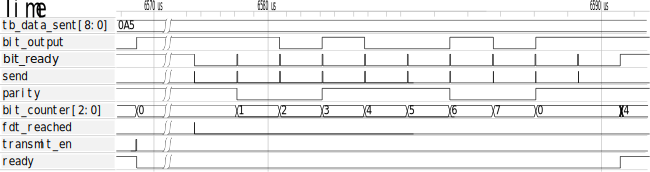
\includegraphics[width=\linewidth]{tb_FrameSender.pdf}
	\caption{Diagrama de tiempos del módulo \lstinline{Frame Sender}.}
	\label{fig:FrameSenderDiagTiempos}
\end{figure}

\begin{figure}
	\centering
	\includegraphics[]{DiagramaEstadosFrameSender}
	\caption{Diagrama de estados del módulo \lstinline{Frame Sender}.}
	\label{fig:FrameSenderDiagEstados}
\end{figure}

Una vez recibida la señal \lstinline{fdt} comienza la transmisión 
direccionando el primer bit con el multiplexor, que siempre es el 
bit de <<Inicio>> de comunicación, y enviando un 
pulso a través de \lstinline{send} al módulo \lstinline{Bit Coder}. 
Este módulo se encarga de codificar el bit y de generar la señal de 
manejo del modulador de carga. 

Cuando \lstinline{Bit Coder} finaliza la transmisión, activa 
la señal \lstinline{bit_ready}, informando que se encuentra disponible 
para enviar otro bit. Al recibir esta señal la máquina de estados 
direcciona el bit siguiente, \(d_{0}\), nuevamente envía un pulso a 
través de \lstinline{send}, y luego espera a que se active la señal 
\lstinline{bit_ready} antes de continuar. Cuando finaliza el envío de 
\(d_{0}\) se continua con \(d_{1}\), luego \(d_{2}\) y así 
sucesivamente.

Como la cantidad de bits en el registro de entrada puede ser menor a 
ocho, el proceso se repite hasta que la cantidad de bits enviados, o lo 
que es lo mismo, la dirección del multiplexor, sea igual a la cantidad 
de bits cargados en \lstinline{Tx Buffer}. Cuando esto se cumple se 
pasa automáticamente a la dirección del bit de paridad \(P\). En caso 
contrario,  
se continúa incrementando la dirección hasta enviar todos los bits y 
llegar a \(P\), lo que sucederá cada vez que se envíe una trama 
estándar con ocho bits de datos.

El bit de paridad se calcula del mismo modo que en el módulo 
\lstinline{Frame Receiver}, sólo que en este caso se utilizan para 
el cálculo los bits de salida del multiplexor. Al finalizar la 
transmisión del bit de <<Inicio>>, el bloque generador de paridad es 
reiniciado por la máquina de estados. Luego, a medida que los bits 
de datos son seleccionados, se hacen ingresar al generador hasta que 
finalmente, cuando se selecciona \(P\), se toma su salida y se envía 
en la posición del bit de paridad. De esta forma se cumple siempre el 
requerimiento del estándar de enviar los datos con paridad impar.

Por último, cuando \lstinline{Bit Coder} informa que finalizó
la transmisión del último bit, la máquina de estados activa la señal 
\lstinline{ready} que informa al circuito o dispositivo externo que finalizó la 
transmisión. Esto sucede en realidad un ciclo de reloj antes de que el 
último bit termine y permite que, en caso de recibir una nueva orden de 
transmisión durante el ciclo de reloj siguiente a la activación de 
\lstinline{ready}, se continúe la trama enviando un nuevo bloque de 
datos más paridad sin bit de <<Inicio>>. Cuando esto ocurre, se cargan
los registros de entrada con los datos de \lstinline{Tx Buffer}, se 
direcciona directamente el bit \(d_{0}\) y se repite el proceso de 
envío.

Si \lstinline{transmit} no se activa durante el ciclo de reloj 
siguiente al flanco ascendente de \lstinline{ready}, la trama se 
da por terminada y la máquina de estados vuelve al estado de reposo.


\subsection{Módulo \lstinline{Bit Coder}}

\begin{figure}
	\centering
	\includegraphics[]{BitCoder}
	\caption{Diagrama del módulo \lstinline{Bit Coder}.}
	\label{fig:BitCoderDiagBloques}
\end{figure}

El módulo \lstinline{Bit Coder} se encarga de codificar los bits que 
deben ser enviados a través de la interfaz de RF como especifica el 
estándar (ver tabla \ref{tab:CodificacionPICC_PCD}) y generar la señal 
de comando del modulador de carga. 

En la figura \ref{fig:BitCoderDiagBloques} se muestra un diagrama de 
los componentes internos del módulo. Allí se observa que el mismo 
está compuesto por un bloque codificador \emph{Manchester}, un 
divisor de frecuencia y una compuerta AND. La salida \lstinline 
{coded_out} es la señal de comando de la llave que conecta la carga 
en el bloque modulador analógico. Cuando \lstinline{coded_out} es 
igual a `1' la llave se cierra y por lo tanto se dice que la 
portadora está \emph{cargada}. Por otro lado, cuando 
\lstinline {coded_out} es `0' la llave está abierta y no se carga a 
la señal de RF.

El Codificador Manchester se encarga de generar el código  
a partir de los bits de entrada. En el estado de reposo su salida se 
mantiene en `0' y por lo tanto la salida del módulo 
\lstinline{coded_out} también. Al recibir un pulso en la entrada 
\lstinline{send} produce en su salida el código Manchester 
correspondiente al estado de \lstinline{bit_in}. Cada bit codificado 
tiene la duración especificada por el estándar, es decir, 128 ciclos 
de reloj. Al finalizar con el código activa la señal 
\lstinline{ready} y vuelve al estado de reposo.

Por otro lado, el divisor de frecuencia divide la señal de reloj de 
\SI{13.56}{\mega\hertz} por 16 para generar la señal sub-portadora 
de \SI{848}{\kilo\hertz}. El estándar especifica que la modulación 
de carga al inicio de cada bit debe tener una fase definida, es por 
ello que se incluyó en el divisor de frecuencia la entrada 
\lstinline {init}. Según la norma, los bits deben comenzar con el 
estado \emph{cargado} de la señal de RF y entonces la entrada 
\lstinline{init} sirve para forzar el estado de la salida del divisor 
de frecuencia a `1' cada vez que comienza la transmisión de un bit.

Finalmente, la operación AND de los bits codificados en código 
Manchester con la señal sub-portadora da como resultado las secuencias 
definidas en la tabla \ref{tab:CodificacionPICC_PCD}. 

Un detalle importante es que \lstinline{Bit Coder} informa que finalizó
la transmisión de un bit un ciclo antes de que la transmisión 
realmente termine. Esto es debido a que se debe permitir continuar 
la con la trama con un nuevo pulso en \lstinline{send} sin 
interrumpirla ni dejar espacios entre bits. 


\section{Verificación funcional}

La verificación del funcionamiento fue realizada módulo por módulo y 
luego del sistema completo utilizando para ello el conexionado que 
realiza el eco de un byte.

Los \emph{testbenchs}\footnote{Bancos de prueba codificados en lenguaje
\emph{Verilog}} desarrollados permitieron generar las señales de 
entrada del sistema digital y enviar datos con tan solo llamar a un 
\emph{task} de \emph{Verilog}, pasando como argumento el valor a 
enviar. 

Los \emph{tasks} de más bajo nivel generan el patrón de envolvente de 
la portadora correspondiente a las secuencias X, Y o Z. El patrón de 
envolvente se utiliza para generar la señal \lstinline{pause} y a la 
vez, a través de una operación AND lógica, se detiene el reloj del 
sistema. De esta forma se simula lo que sucede realmente al arribar 
una pausa en la portadora. También se codificaron \emph{tasks} para 
generar las secuencias de <<Inicio>> y <<Fin>> de comunicación y luego 
se escribió un \emph{task} de más alto nivel que utiliza a los 
anteriores para enviar cualquier bytes de datos pasado como parámetro. 

Con los \emph{tasks} desarrollados se pudieron enviar las tramas de 
entrada al sistema digital y verificar la respuesta del mismo. Para 
probar el sistema de recepción de información se desarrollo un 
\emph{testbench} que envía los bytes de 8'h00 a 8'hFF, de a uno por 
vez y armando la trama completa, es decir, <<Inicio>> + datos + 
<<Paridad>> + <<Fin>> y comprueba automáticamente que a la salida de 
\lstinline{Frame Receiver}, en el registro \lstinline{byte_buf}, quede 
almacenado el valor correcto cuando se genera el pulso en 
\lstinline{new_byte}. Las pruebas realizadas de esta forma permitieron 
depurar el diseño hasta obtener un sistema de recepción de 
información libre de errores.

Por otro lado, para el sistema de transmisión de información el 
\emph{testbench} desarrollado constó del envío de algunos bytes 
típicos, que fueron cargados manualmente en el buffer de transmisión, 
y la verificación se hizo mediante el análisis del diagrama de 
tiempos del sistema. En este caso no se desarrolló un test 
automatizado debido a la dificultad de leer y verificar la señal 
\lstinline{coded_out}, que está formada por el código 
\emph{Manchester} modulado con la sub-portadora, mediante código en 
\emph{Verilog}. Sin embargo, también se hizo la prueba exhaustiva 
de enviar los 256 bytes de datos posibles utilizando para ello el 
conexionado de la interfaz de recepción con la de transmisión, como 
se verá a continuación.

\subsection{Eco de un byte}

En la figura \ref{fig:DigitalBlockDiagram} se muestra en líneas 
punteadas como puede conectarse directamente la salida del bloque
receptor con la entrada del bloque transmisor para obtener un \emph{tag} 
autónomo que realiza el eco de un byte, es decir, devuelve al lector 
el byte de datos recibido. Al conectar el dispositivo de esta forma, 
los bits recibidos en \lstinline{rx_bit} ingresan directamente al 
buffer de transmisión. Al finalizar la trama y detectarse el símbolo 
de <<Fin>> se activa la señal \lstinline{rx_eof}, que a su vez sirve 
de señal de inicio de transmisión a través de \lstinline{tx_transmit}.

El diseño puede retransmitir sólo un byte de datos, ya que el buffer de 
transmisión tiene el tamaño de un byte y se sobreescribe si se recibe una 
cantidad de datos mayor.

En la figura \ref{fig:SimulacionDigital} se muestra una simulación a 
nivel lógico del bloque digital con la conexión que produce el eco. 
Allí se observa como el dispositivo recibe el byte de datos, 8h'53 
en este caso, a la vez que lo carga en el buffer e inicia la 
transmisión luego de cumplido el FDT. Las señales 
\lstinline {tb_rx_bit} y \lstinline{tx_bit} son los bits recibidos y 
a cargar en el buffer, mientras que \lstinline{tb_rx_new_bit} indica 
que el bit es un nuevo bit válido para la lectura y 
\lstinline {tx_new_bit} es la señal que habilita la carga del buffer 
de transmisión en el siguiente flanco ascendente de reloj.

Se debe notar que los bits se reciben en orden \emph{LSB First}, es 
decir, se recibe primero el bit menos significativo. El 
buffer de transmisión fue diseñado para ser cargado también en ese 
orden, lo que evita el uso de componentes externos.

\begin{figure}
	\centering
	\includegraphics[width=\textwidth]{tb_top_phy_layer}
	\caption{Simulación del bloque digital cuando el dispositivo es 
	utilizado en modo \emph{eco}.}
	\label{fig:SimulacionDigital}
\end{figure}

En el \emph{testbench} desarrollado para verificar la funcionalidad 
del modo \emph{eco} se enviaron los 256 bytes de datos posibles al 
sistema digital y todos fueron reenviados a través de 
\lstinline{coded_out} correctamente.

\section{Implementación: Síntesis y \emph{Place\&Route}}

La descripción del hardware en lenguaje \emph{Verilog} fue 
sintetizada utilizando el software \emph{Synopsys Design Compiler} 
\cite{SynopsysDC} junto con la biblioteca de celdas digitales de la 
\emph{Oklahoma State University} (OSU), celdas que fueron diseñadas 
para el proceso de fabricación C5N de \emph{ON Semiconductor}. 

La biblioteca incluye compuertas lógicas NAND, NOR, XOR, inversores, 
AOI, OAI, etc., junto con buffers especiales para el árbol de 
distribución de reloj, multiplexores y flip-flops tipo D disparados 
por flanco \hyphenation{as-cen-den-te/des-cen-den-te}ascendente/descendente. 
Todas las celdas están caracterizadas en cuanto a tiempos de 
propagación para todos los caminos posibles entre entradas y 
salidas, cuentan con características dinámicas de las salidas, como 
son los tiempos de crecimiento/decrecimiento y consumo de potencia 
dinámica según la capacidad de carga.

La herramienta de síntesis utiliza la caracterización de las 
compuertas junto con restricciones impuestas al diseño para 
optimizar los tiempos de retardo y el área ocupada por el circuito. 
La frecuencia de operación es la primer restricción de todo circuito 
sincrónico y en este caso es de \SI{13.56}{\mega\hertz}. Sin embargo, 
para contar con un margen de seguridad en caso de que el retardo de 
las compuertas fuese mayor al esperado por variaciones del proceso, se impuso como restricción una 
frecuencia de operación de \SI{15}{\mega\hertz}. 

Por otro lado, para reducir el consumo de potencia se activó la 
opción de la herramienta de síntesis que hace uso de la técnica 
\emph{clock gating}. Esta técnica agrega una pequeña lógica en la entrada 
de reloj de los flip-flops que permite activar o desactivar esa señal. 
Cuando un FF debe mantener el estado de su salida durante varios ciclos
de reloj, como por ejemplo los FF siguientes al primero de un contador 
binario, se desactiva la señal de reloj en su entrada para evitar el consumo de 
potencia dinámica debido a la transición del reloj de un estado a otro.

El trazado físico del diseño (\emph{Place\&Route}) se realizó con el 
software \emph{Synopsys IC Compiler} \cite{SynopsysICCompiler}. En 
este caso se le debe indicar al programa la forma o tamaño deseado. 
Como el área ocupada en general se desea que sea la mínima posible, 
se suele definir entonces la relación de aspecto alto/ancho del 
trazado deseado. También se le deben indicar las posiciones de las 
entradas y salidas del bloque, que luego serán conectadas con el resto 
del los circuitos. 

El programa ubica las compuertas optimizando las 
posiciones según el conexionado. Luego genera un árbol de reloj y 
finalmente realiza el conexionado de todas las compuertas. El 
\emph{layout} final del bloque digital puede verse en la figura 
\ref{fig:LayoutBloqueDigital}.

\begin{figure}
	\centering
	\includegraphics[width=\linewidth]{Layout_digital}
	\caption{\emph{Layout} final del bloque digital. Sus dimensiones 
	son de \SI{900}{\micro\meter} \(\times\) \SI{330}{\micro\meter}.}
	\label{fig:LayoutBloqueDigital}
\end{figure}

Las herramientas generan una serie de reportes del área ocupada, el 
tiempo de retardo del camino crítico y los registros en que se 
utilizó la técnica de \emph{clock gating}. En la tabla 
\ref{tab:AreaDigital} se presenta un resumen del área ocupada por cada 
uno de los módulos del diseño luego de la síntesis lógica y sin 
tener en cuenta el árbol de distribución de reloj ni el área 
necesaria para el conexionado de las compuertas. El módulo 
\lstinline{frame_sender} es el de mayor tamaño, mientras que los 
demás son de tamaños similares, salvo \lstinline{pause_latch} y 
\lstinline{rst_sync}\footnote{Este módulo es el circuito sincronizador 
de la señal de reset.}, que al contener un registro el primero y dos el 
segundo son de tamaño despreciable. 

\begin{table}
	\centering
	\begin{tabu}{lc}
		\toprule
		Módulo & Area \(\left[\si{\micro\meter\squared}\right]\) \\  
		\midrule
		\lstinline{bit_coder}              & 33669 \((15.1\%\)) \\
		\lstinline{bit_decoder}            & 37791 \((16.9\%\)) \\
		\lstinline{frame_delay_counter}    & 28656 \((12.8\%)\) \\
		\lstinline{frame_receiver}         & 36972 \((16.6\%)\) \\
		\lstinline{frame_sender}           & 57447 \((25.8\%)\) \\
		\lstinline{pause_latch}            & 1800  \((0.1\%)\) \\
		\lstinline{rst_sync}     & 3600  \((0.2\%)\) \\
		\lstinline{tx_buffer}              & 22563 \((10.1\%)\) \\
		\midrule
		Total 8 Módulos        &         222498\\
		\bottomrule
	\end{tabu}
	
	\caption{Área utilizada por cada uno de los módulos luego de la 
	síntesis.}
	
	\label{tab:AreaDigital}
\end{table}

En la tabla \ref{tab:ResumenClockGating} puede verse un resumen del 
reporte de la herramienta de síntesis luego de aplicar la técnica 
de \emph{clock gating}. De los 95 registros del diseño, a 70 
se les pudo aplicar esta técnica para reducir el consumo. El software 
también estima la potencia consumida por las compuertas trabajando a 
la frecuencia establecida. Luego de aplicar la técnica de \emph{clock 
gating} la potencia dinámica estimada por el sintetizador se redujo 
un 30\%, de \SI{3.43}{\milli\watt} a \SI{2.39}{\milli\watt}.

Sin embargo, el agregado de las celdas de \emph{clock gating}, cuyo 
esquemático puede verse en la figura \ref{fig:CeldaClockGating}, tiene 
el inconveniente de que disminuye el tiempo disponible para el arribo 
de la señal proveniente de la lógica. Esto es debido a que el latch 
del esquemático actúa cuando el reloj está en nivel bajo, mientras que 
los flip--flops del resto del diseño trabajan por flanco ascendente. 
Entonces, luego de un flanco ascendente de reloj, la entrada 
\lstinline{Gate} tiene sólo medio período para establecerse antes de 
que actúe el latch en el siguiente nivel bajo. Esto afectará el 
camino crítico como se verá a continuación.

\begin{figure}
	\centering
	\includegraphics[]{ClockGatingCell}
	\caption{Celda de \emph{clock gating} construida por el 
	sintetizador.}
	\label{fig:CeldaClockGating}
\end{figure}

\begin{table}
	\centering
	\begin{tabu}{lc}
		\toprule
		\multicolumn{2}{c}{Resumen de \emph{Clock Gating}} \\
		\midrule
		Cantidad total de registros                   &      95      \\
		Cantidad de celdas de \emph{clock gating}  & 13           \\
		Cantidad de registros con \emph{clock gating} & 70 \((73.68\%)\) \\
		Cantidad de registros sin \emph{clock gating} & 25 \((26.32\%)\) \\
		\bottomrule
	\end{tabu}
	
	\caption{Resultado arrojado por la herramienta de síntesis luego de
	aplicar la técnica de \emph{clock gating} al diseño.}
	
	\label{tab:ResumenClockGating}
\end{table}

Finalmente, utilizando las características de retardos y capacidad de 
entradas y salidas, la herramienta calcula el retardo de las señales 
entre registros para ver que se cumpla con la frecuencia de operación 
requerida. En caso de que el retardo sea mayor al período de reloj el 
software optimiza las dimensiones de las compuertas o agrega buffers, 
incrementando el área ocupada, para intentar cumplir con la frecuencia de 
operación indicada. El parámetro que se toma como referencia para 
saber si se cumple o no es el \emph{slack time}, que es el tiempo 
entre que arriba la señal de datos a la entrada de un registro hasta 
que arriba el flanco de reloj. Si el \emph{slack time} fuese negativo 
el circuito no podría funcionar. Luego de la síntesis se genera un 
informe con los tiempos de retardo de cada uno de los caminos posibles 
entre registros. Al camino con menor \emph{slack time} se lo denomina 
\emph{camino crítico} y es el primero que debe optimizarse. 

En la tabla \ref{tab:DigitalCaminoCritico} se muestra el reporte del 
camino crítico para el diseño. El camino parte de la entrada 
\lstinline{tx_transmit} y termina en un FF del módulo 
\lstinline{Frame Sender}. Una de las restricciones impuestas para 
forzar un peor caso es que todas las entradas tengan un retardo de 
\SI{10}{\nano\second} y por este motivo es que en la tabla el 
\emph{input delay} comienza con ese valor. El software suma el retardo 
de las compuertas hasta llegar al registro al final del camino. El 
\emph{data arrival time} es el resultado de la suma, que se compara con el
\emph{data required time} generalmente dado por la frecuencia de trabajo. 
Debido a la utilización de las celdas de \emph{clock gating}, que como 
se dijo reducen el tiempo disponible para el establecimiento de la 
lógica, el \emph{data required time} fue de la mitad del período de 
reloj. Finalmente, el \emph{slack} calculado para el camino crítico fue de 
\SI{22.18}{\nano\second} y no fue necesario intervenir en la síntesis.

\begin{table}
	\centering
	\begin{tabu}{lc}
		\toprule
		Punto            & Retardo \(\left[\si{\nano\second}\right]\) \\
		\midrule
		Input external delay        &   10.00 \\
		frsen/U13/Y (INVX2)         &   10.07 \\
		frsen/U65/Y (NOR2X1)        &   10.28 \\
		frsen/U74/Y (NAND2X1)       &   10.70 \\
		frsen/U81/Y (OAI22X1)       &   10.82 \\
		Data arrival time           &   10.82 \\
		\addlinespace
		Clock clk' (rise edge)      &   33.00 \\
		Clock network delay (ideal) &   33.00 \\
		\midrule
		Data required time          &   33.00 \\
		Data arrival time           &  -10.82 \\
		\midrule
		Slack (MET)                 &   22.18 \\
		\bottomrule
	\end{tabu}
	
	\caption{Retardos del camino crítico: Desde \lstinline{tx_transmit} 
	hasta \lstinline{frsen/clk_gate_bits_to_send_ret_reg/latch}.} 
	%\footnote{\lstinline{frsen} es \lstinline{frame_sender}}.}
	
	\label{tab:DigitalCaminoCritico}
\end{table}

Luego, mediante una simulación a nivel de transistor se obtuvo la 
corriente promedio de consumo del bloque digital, que fue de 
\SI{325}{\micro\ampere} a \SI{3}{\volt}, lo que da una potencia 
ligeramente menor a la estimada por el sintetizador.
